\chapter{Antecedentes}

Aunque la definición de IoT puede variar dependiendo del autor, según la recomendación de la Unión Internacional de Telecomunicaciones (ITU, siglas en inglés de \textit{International Telecommunication Union}), IoT puede definirse como una infraestructura que facilita la prestación de servicios a través de la conexión de objetos físicos y virtuales, utilizando las tecnologías de la información y comunicación que permita interoperabilidad de los sistemas actuales o futuros. Es decir, una evolución de Internet desde una red de computadoras hasta una red de objetos interconectados (\citep{itu2014}).

\vspace{0.5cm}

El concepto de IoT fue utilizado por primera vez por el pionero en tecnología Kevin Ashton en una presentación que realizó para Procter \& Gamble en 1999 en donde describe un sistema en el cual objetos del mundo físico podrían conectarse a Internet a través de sensores para automatizar la recolección de datos, básicamente destacaba cómo la información de la cadena de suministro, cuando es capturada de forma manual por las personas, es propensa a retrasos y errores de captura; sin embargo, si se introducía directamente desde los objetos, se podía tener información en tiempo real, aumentar la productividad y reducir gastos operativos (\cite{ashton2009}).

\vspace{0.5cm}

En consecuencia, cualquier objeto puede ser una fuente de datos e incorporarse al IoT. Las aplicaciones para IoT son numerosas y diversas, incorporándose cada vez más a todas las áreas de la vida cotidiana.

\section{Nodo IoT}

Un nodo IoT es un dispositivo de hardware capaz de detectar fenómenos físicos mediante sensores que miden variables de forma analógica o discreta, preprocesa esta información y la comparte. Este forma parte de una red de IoT y se encarga de monitorear la ocurrencia de eventos de manera pasiva y continua. Dependiendo de su aplicación, un nodo IoT notifica sus valores utilizando dos enfoques principales: transmisión basada en eventos o notificación continua.

\vspace{0.5cm}

La transmisión basada en eventos ocurre cuando el nodo informa únicamente al detectarse un evento relevante, como una lectura específica del sensor o el cumplimiento de un temporizador. Por otro lado, la notificación continua implica que cada lectura realizada por el sensor se transmite en tiempo real (\cite{caldas2020}).

\begin{figure}
    \centering
    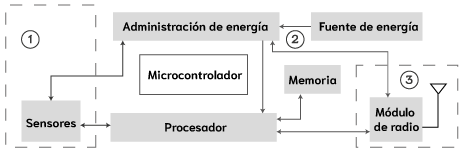
\includegraphics[width=0.60\linewidth]{tesis_fvalde/Imagenes/Nodo-IoT.png}
    \caption{Arquitectura de un nodo IoT}
    \label{fig:nodo_iot}
\end{figure}

\vspace{0.5cm}

El propósito principal de un nodo IoT es recolectar, procesar y transmitir datos hacia otros dispositivos o servidores. Para cumplir esta función según (\cite{bouguera2018}) y para optimizar su vida útil, los nodos IoT están compuestos por tres unidades principales: la unidad de sensor (1), la unidad de procesamiento (2) y el módulo de radio (3) según puede observarse en la Figura 2.1. Estas unidades trabajan en conjunto para garantizar la eficiencia energética, el cual es un factor crítico en la vida útil de estos dispositivos, estas se describen a continuación:


\begin{itemize}
   \item Unidad del sensor. La señal de entrada es generalmente una señal analógica que se convierte a digital con un convertidor analógico a digital (ADC, las siglas en inglés de \textit{Analog to Digital Converter}).
   \item Unidad de procesamiento. Administra todos los recursos del sistema.
   \item Unidad de comunicación. Una vez que se realiza el procesamiento de datos, la información se debe enviar a un punto de acceso.
\end{itemize}

\section{Redes de área amplia de baja potencia}

Aunque IoT involucra distintas clases de redes, una de las principales son las Redes de Area Amplia de Baja Potencia (LPWAN, las siglas en inglés de \textit{Low Power Wide Area Network}), que varían en el alcance de la señal y la velocidad máxima de transmisión. La cobertura de la señal en LPWAN suele ser de varios kilómetros y su velocidad se expresa en kilobits por segundo (Kbps) (\cite{Herrero2023}). 

\vspace{0.5cm}

Las redes LPWAN son redes de telecomunicaciones destinadas al envío de pequeños paquetes de datos, con un bajo consumo de energía que permita a dispositivos IoT operar durante largo tiempo sin necesidad de recargar o cambiar baterías.

\vspace{0.5cm}

En la Tabla 2.1 se muestra una comparación de LoRa con otras tecnologías inalámbricas.

\begin{table}[h!]
    \centering
    \caption{Comparación de Bluetooth y Zigbee con LoRa}
    \begin{tabular}{p{6cm}p{3cm}p{3cm}p{3cm}}
        \toprule
        \textbf{} & \textbf{LoRa} & \textbf{Zigbee} & \textbf{Bluetooth} \\
        \midrule
        \textbf{Topología} & Estrella & Malla, Estrella & Estrella \\
        \textbf{Duración de la batería} & Décadas & Años & Días \\
        \textbf{Velocidad máxima} & 50 kbps & 250 Kbps & 1 Mbps \\
        \textbf{Cobertura} & 5-15 km & 70-300 m & 100 m \\
        \bottomrule
    \end{tabular}
    \label{tab:comparison}
\end{table}

\section{LoRa}

La tecnología LoRa (abreviatura en inglés de \textit{Long Range}) fue desarrollada por una empresa francesa llamada Cycleo y, posteriormente, adquirida y patentada por Semtech. Esta compañía comercializa los módulos de radio LoRa, los cuales utilizan un protocolo que proporciona comunicación LPWAN para el envío de pequeños paquetes de datos a largas distancias con una potencia de señal baja a un bajo consumo de energía, permitiendo que los dispositivos compatibles funcionen hasta 10 años con una sola batería (\cite{augustin2016}).

\vspace{0.5cm}

La capa física de LoRa opera en las bandas de espectro de radio sin licencia en la banda de Radio Industrial, Científica y Médica (ISM, siglas en inglés de \textit{Industrial, Scientific, and Medical}) de 433 MHz y 915/868 MHz. Algunas bandas de frecuencia ISM se muestran a continuación:

\begin{itemize}
  \item Estados Unidos y México: 902-928 MHz
  \item Unión Europea: 863-870 y 433 MHz
  \item China: 779-787, 433,575 MHz
  \item Australia: 915-928 MHz
  \item Asia: 923 MHz
  \item Corea del Sur: 920-923 MHz
  \item India: 865-867 MHz
\end{itemize}

\vspace{0.5cm}

LoRa emplea la modulación CSS (siglas en inglés de \textit{Chirp Spread Spectrum}). CSS es una tecnología de espectro extendido de banda ancha. Esta técnica implica una modulación en la que la frecuencia de la señal varía, aumentando o disminuyendo con el tiempo dentro del ancho de banda disponible. CSS no solo optimiza el consumo energético, sino que también permite transmisiones de largo alcance llegando hasta 10 km con velocidades de transmisión bastante bajas (\cite{Herrero2023}).

\vspace{0.5cm}

En LoRa un \textit{chirp} es una señal cuya frecuencia aumenta (\textit{upchirp}) o disminuye (\textit{downchirp}) de manera lineal durante un intervalo de tiempo definido. Los \textit{chirps} son la base de la modulación CSS en LoRa, que permite la transmisión de datos con alta inmunidad al ruido y robustez en largas distancias. Los \textit{downchirps} tienen roles específicos en las comunicaciones LoRa, como en las señales de sincronización y el proceso de recepción de paquetes.

\vspace{0.5cm}

Las redes LoRa se utilizan ampliamente para aplicaciones LPWAN porque permite la configuración de redes autónomas a bajo costo. Las redes LoRa se han implementado para muchos sistemas de investigación y aplicaciones IoT como edificios inteligentes, ciudades inteligentes, agricultura inteligente, medidores inteligentes y medidores de calidad del agua (\cite{sundaram2019}).

\vspace{0.5cm}

\begin{figure}[h]
    \centering
    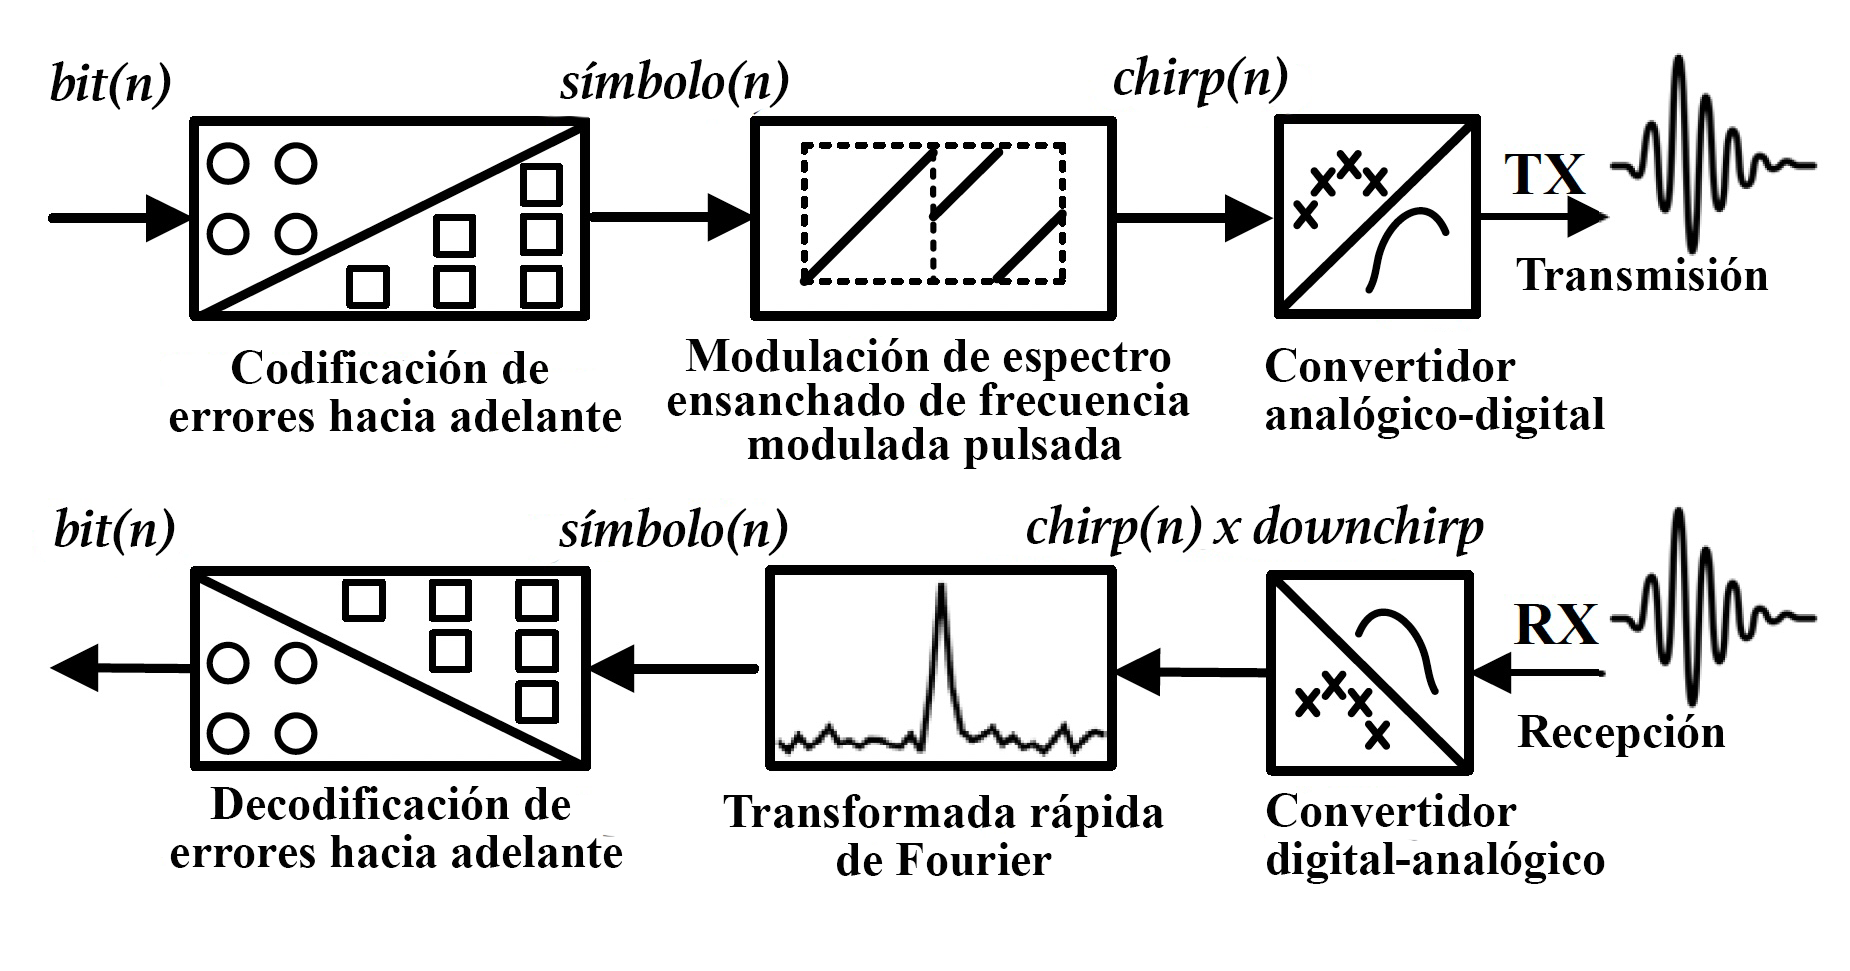
\includegraphics[width=0.5\linewidth]{tesis_fvalde/Imagenes/lora_phy.png}
    \caption{Capa física de LoRa}
    \label{fig:lora_phy}
\end{figure}

La Figura 2.2 ilustra la capa física de LoRa PHY (abreviatura en inglés de \textit{Physical Layer}) y el flujo de trabajo de TX/RX. En el TX, los flujos de bits entrantes de la capa superior se codifican primero en símbolos LoRa redundantes mediante codificación de canal. Luego, los símbolos LoRa se modulan en \textit{chirps}, se convierten en señal de banda base analógica por el DAC y se modulan en la frecuencia portadora. Para recibir un paquete LoRa, el RX convierte de manera descendente la señal recibida en señal de banda base y la muestrea con el ADC. Después, los \textit{chirps} LoRa se demodulan en dos pasos: (1) multiplicación con un chirp descendente (\textit{downchirp}) estándar predefinido, y (2) realización de la Transformada Rápida de Fourier (FFT, siglas en inglés de \textit{Fast Fourier Transform}) en el producto resultante.  Por último, el decodificador transforma el símbolo LoRa en bits originales revirtiendo el proceso de codificación del canal. 

\subsection{Parámetros}

La capa física de LoRa se caracteriza por varios parámetros, entre los que destacan la frecuencia (CF, siglas en inglés de \textit{Carrier Frequency}), el ancho de banda (BW, siglas en inglés de \textit{Bandwidth}), el factor de esparcimiento (SF, siglas en inglés de \textit{Speading Factor}) y la tasa de codificación (CR, siglas en inglés de \textit{Coding Rate}) (\cite{wang2020}). La combinación de estos parámetros proporciona diferentes valores de energía y rangos de transmisión (\cite{bouguera2018}), estos parámetros son:

\begin{itemize}
   \item Frecuencia (CF): es la frecuencia central para la banda de transmisión. Esta puede ser 433 MHz, 863 a 870 MHz en Europa y 915 MHz para América.
   
   \item Ancho de banda (BW): representa el rango de frecuencias de la banda de transmisión. Se elige entre tres valores: 125 kHz, 250 kHz o 500 kHz. La distancia del enlace es en función del ancho de banda y SF.
   \item Tasa de codificación (CR): El CR puede variar entre 4/5 y 4/8. Esto implica que, por cada 4 bits de datos enviados, se agregan de 1 a 4 bits adicionales para la detección y corrección de errores. Cuanto menor sea la tasa de codificación, mayor será el tiempo que se tarde en transmitir los datos en el aire. CR es igual a $\frac{4}{4 + n}$ donde n es un valor de 1 a 4. 
   \item Factor de esparcimiento (SF): es el número de \textit{chirps} por símbolo. Su valor es un número entero entre 7 y 12.
   \\
   \\
   La Tabla 2.2 presenta las velocidades de bits calculadas con SF7 y CR = 1 para anchos de banda de 125, 250 y 500 kHz.\\

\end{itemize}

\begin{table}[h!]
    \centering
    \caption{Tabla de factores de esparcimiento, ancho de banda y velocidad de bits}
    \begin{tabular}{p{3cm}p{3cm}p{6cm}}
        \toprule
        \textbf{SF} & \textbf{BW} & \textbf{Velocidad de bits (kbits/s)} \\ 
        \midrule
        7 & 125 & 5.5 \\ 
        7 & 250 & 10.9 \\ 
        7 & 500 & 21.9 \\ 
        \bottomrule
    \end{tabular}
    \label{tab:table_sfx}
\end{table}

\subsection{Estructura de la trama}

Una trama de red LoRa tiene varias secciones. La trama del paquete LoRa comienza con un preámbulo, la longitud del preámbulo es variable. Después del preámbulo sigue una cabecera opcional que puede ser explícita (incluida en el paquete) o implícita (omitida para reducir el tamaño del paquete, pero requiere que el receptor y el transmisor estén configurados previamente) (\cite{bouguera2018}). Luego de la cabecera viene el paquete de datos o carga útil que puede oscilar entre 11-252 bytes (\cite{morales2021}). 

\begin{itemize}
   \item Preámbulo: es la primer parte de la trama, el valor predeterminado es 8 pero su longitud puede variar de 6 a 6553 valores. Su función es facilitar la sincronización entre el transmisor y el receptor.
   \item Cabecera: contiene información como la longitud del paquete, presencia o ausencia de la verificación de redundancia cíclica (CRC, siglas en inglés de Cyclic Redundancy Check).
   \item Datos: es el contenido principal del paquete.
   \item CRC: Es una suma de comprobación opcional que asegura que los datos no se corrompieron durante la transmisión.
\end{itemize}

\vspace{0.5cm}

El tamaño máximo de paquete de datos depende de varios factores, incluyendo el BW y el SF, ya que el aumento de estos reduce la tasa de transmisión efectiva y, en algunos casos, el límite del paquete de datos.

\vspace{0.5cm}

\begin{figure}[h]
    \centering
    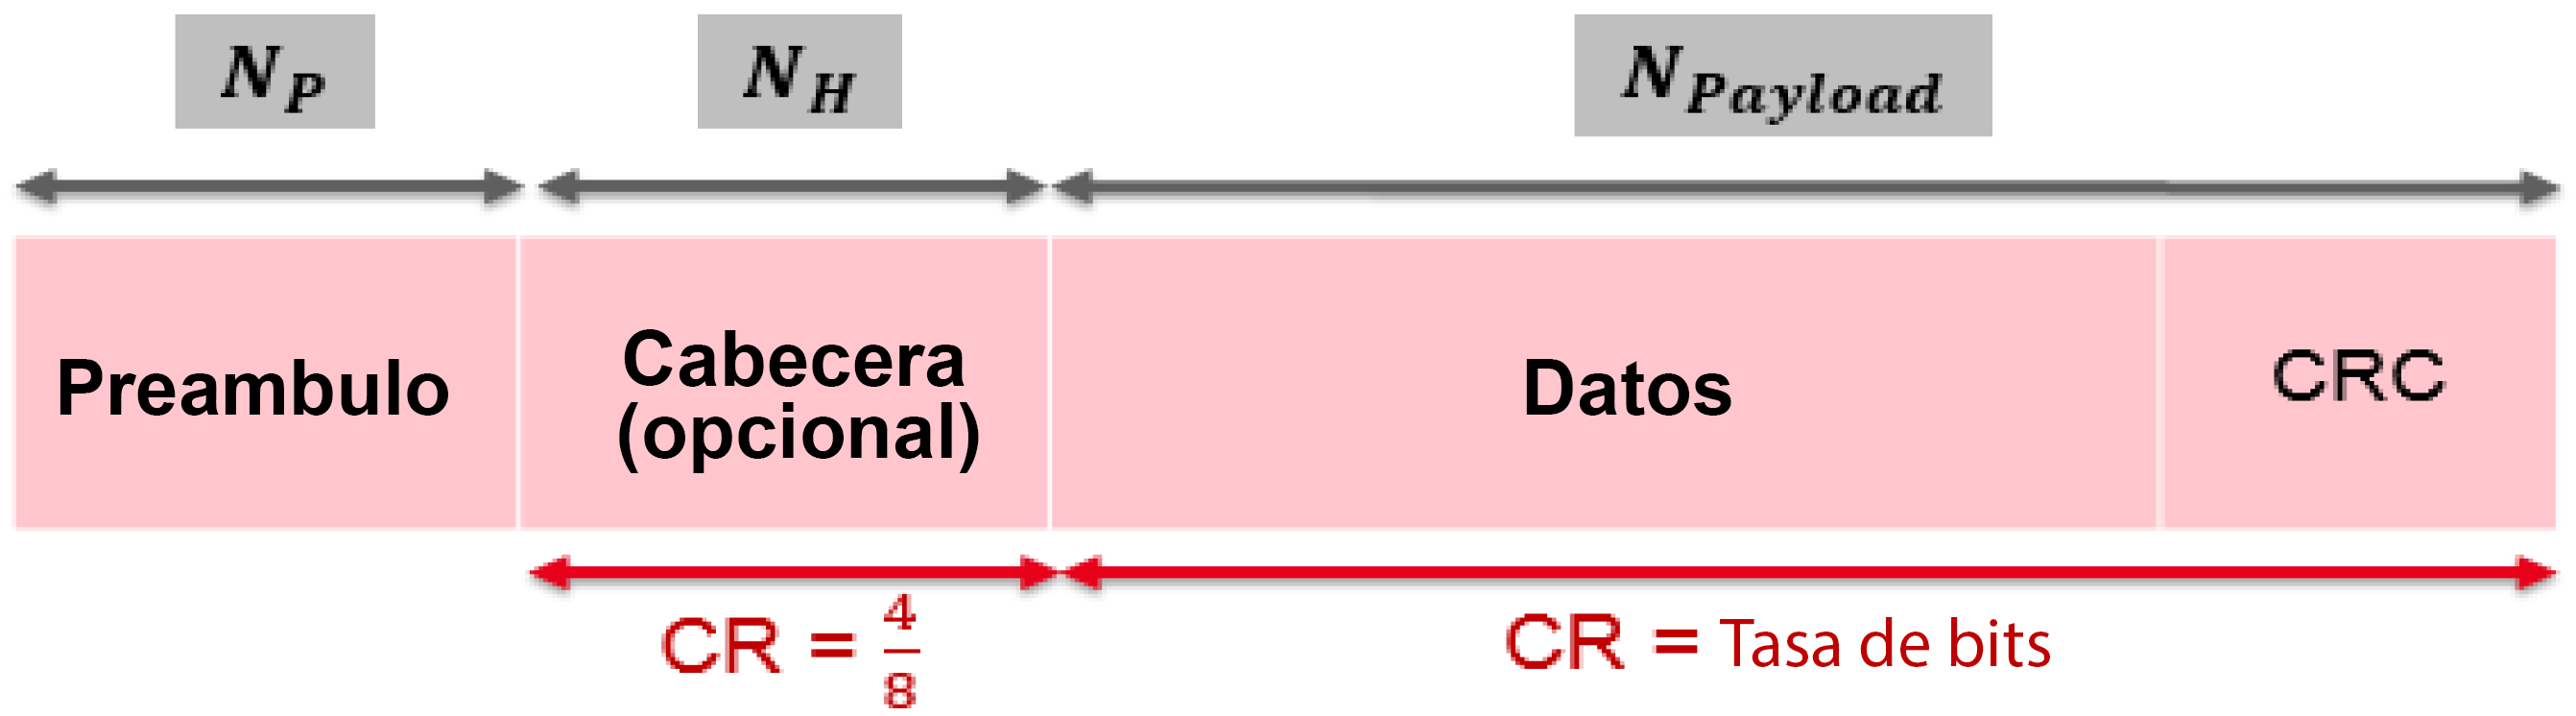
\includegraphics[width=0.50\linewidth]{tesis_fvalde/Imagenes/estructura_paquete.png}
    \caption{Estructura de trama de red LoRa}
    \label{fig:estructura_paquete}
\end{figure}

Como se observa en la Figura 2.3, la información está codificada con un CR variable, sin embargo la cabecera siempre está codificada con un $CR = \frac{4}{8}$. Adicionalmente se puede incluir de manera opcional un código de redundancia CRC al final del paquete. 

\section{LoRaWAN}

El protocolo LoRaWAN fue desarrollado por LoRa Alliance, y la capa física y modulación inalámbrica de largo alcance LoRa está patentada por Semtech. 

\vspace{0.5cm}

La Figura 2.4 ilustra la estructura en cuatro capas del estándar LoRaWAN. En esta arquitectura, los dispositivos finales se conectan a la red a través de pasarelas de red o GW (abreviatura del inglés \textit{gateways}). Estos últimos, dispositivos de interconexión entre redes con protocolos y arquitecturas diferentes emplean la modulación LoRa para recibir los datos de los sensores y actuadores, y los transmiten a un servidor central en una topología en estrella.

\vspace{0.5cm}

Finalmente, los servidores de aplicación son los responsables de procesar, administrar e interpretar los datos recibidos desde los nodos, así como asegurar la autenticidad de cada mensaje recibido y la integridad de los mismos (\cite{10.1007/978-3-031-08878-0_6}). Las funciones principales del servidor de red LoRaWAN (\cite{estrada2019diseno}) son:

\begin{figure}[h]
    \centering
    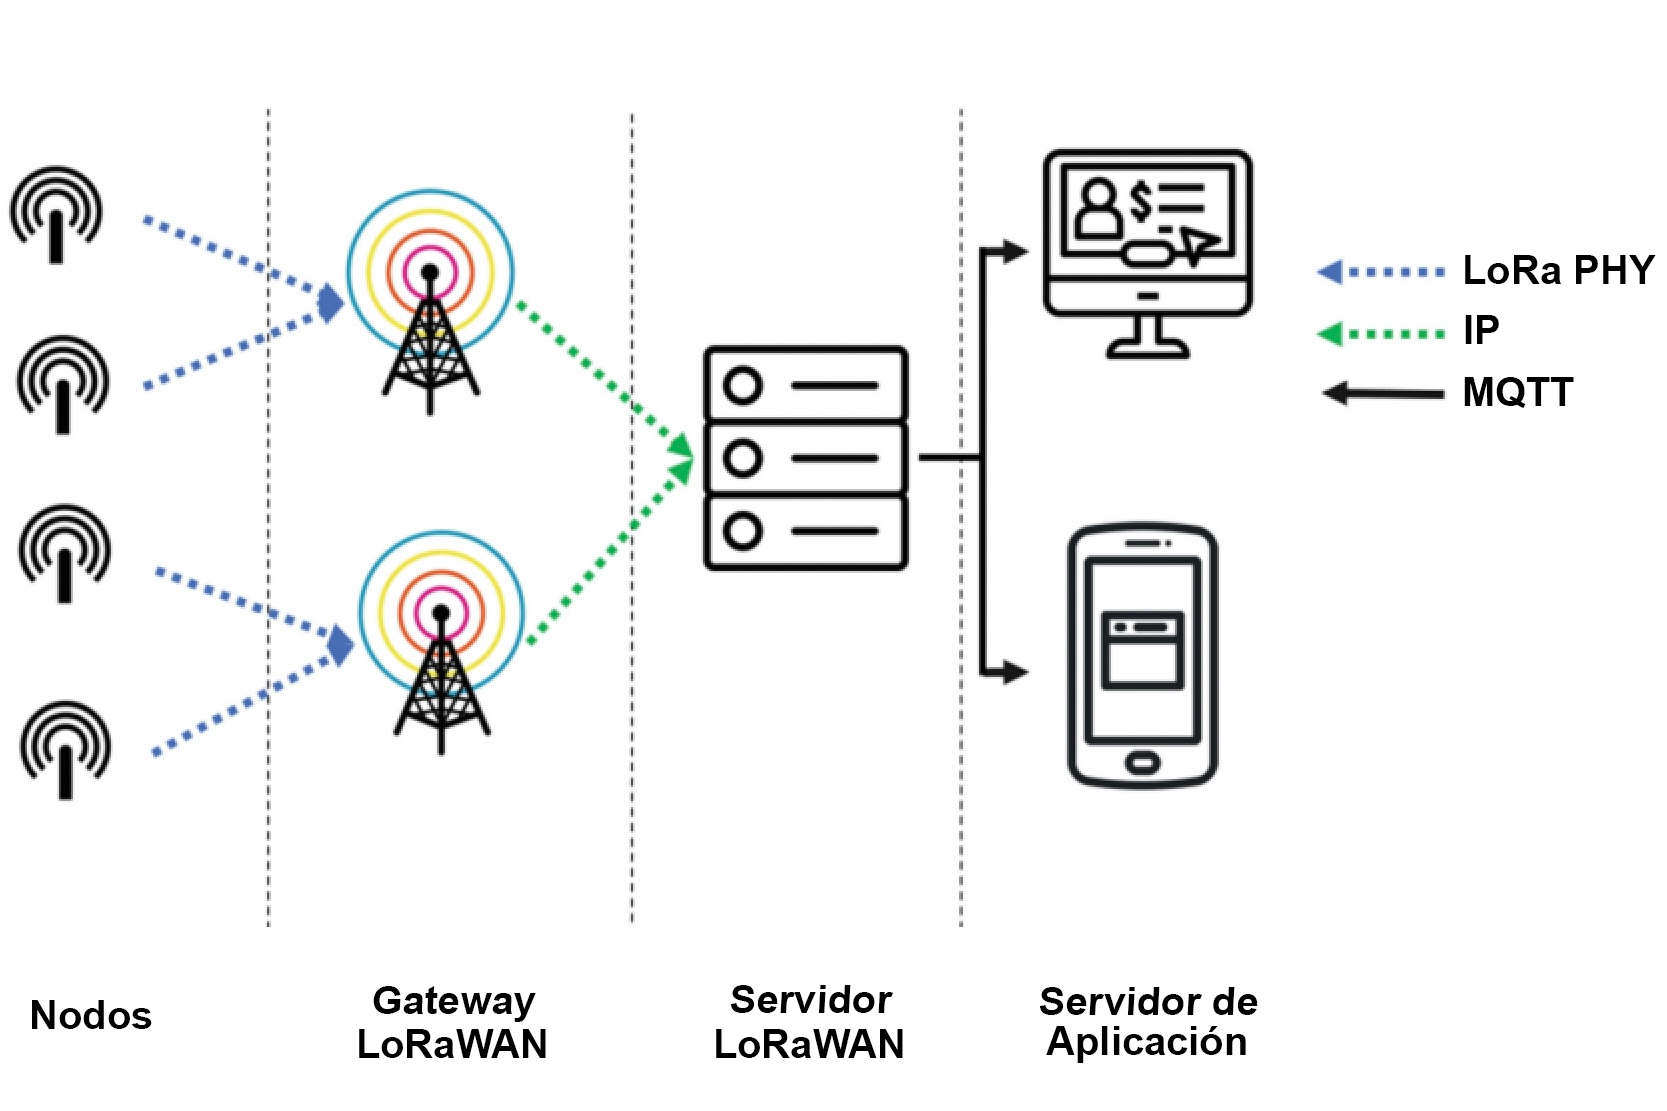
\includegraphics[width=0.65\linewidth]{tesis_fvalde/Imagenes/arquitectura-lorawan.png}
    \caption{Arquitectura LoRaWAN}
    \label{fig:arquitectura_lorawan}
\end{figure}

\begin{itemize}
    \item Activación de dispositivos: El servidor es el encargado de dar la bienvenida a nuevos dispositivos a la red.
    \item Prevención de duplicados: Evita que se procesen múltiples veces los mismos datos recibidos desde diferentes GW.
    \item Enrutamiento: Selecciona la ruta para que los datos lleguen a su destino.
    \item Reenvío de datos: Transmite los datos de los dispositivos a los servidores de aplicaciones correspondientes.
    \item Administración de la red: Realiza tareas de mantenimiento y configuración de la red en general, como el ajuste de parámetros de los dispositivos y la generación de informes.
\end{itemize}

En LoRaWAN son los GW los que están conectados a Internet, no los nodos, ya que estos solo recopilan los datos para los que fueron diseñados (\cite{morales2021}).

\section{The Things Network (TTN)}

TTN es una red LoRaWAN que facilita el registro de GW, aplicaciones y dispositivos (nodos), así como la transmisión de datos desde los nodos al servidor de red a través de las puertas de enlace registradas. 

\vspace{0.5cm}

TTN tiene algunas restricciones como son: transmitir solo datos binarios, mantener el tamaño de los datos lo más pequeño posible o evitar la transmisión continua de datos (\cite{thasjohn2023arduino}). Además, el diseño de hardware de sus gateways, nodos y código está disponible libremente en Internet como código abierto. Las condiciones de uso se plasmaron en un manifiesto en el que se pueden destacar (\cite{escribano2021sistema}):

\begin{itemize}
    \item Cualquiera podrá configurar un nodo a través de un GW perteneciente a TTN.
    \item Cualquiera podrá configurar un GW y unirse a la red TTN.
    \item El acceso a los nodos es neutral y todos reciben el mismo trato en la red.
    \item Cualquiera que implemente un GW en la red TTN lo hará de forma gratuita.
    \item Cualquiera puede hacer uso de la red TTN.
    \item Los datos que se generan en los nodos son propiedad del usuario y no son accesibles por nadie más.
\end{itemize}

A lo largo de los años la comunidad TTN ha crecido de tal manera que existen GW disponibles en más de 136 países del mundo con más de 7,000 usuarios y más de 7,300 GW.

\section{Bus SPI}

El Bus SPI o interfaz de comunicación serial SPI (siglas en inglés de \textit{Serial Peripheral Interface}) es un estándar de comunicación en serie, es decir, que los bits que conforman la transmisión, se envían uno tras otro por un mismo puerto. Fue estandarizado por Motorola para su primer microcontrolador y está basado en la existencia de un único dispositivo maestro (un solo dispositivo es el responsable de iniciar todas la comunicaciones con el resto de periféricos y/o sensores, denominados esclavos). La sincronización y la transmisión de datos se realiza por medio de 4 señales:

\begin{itemize}
    \item Señal de reloj o SCLK (abreviatura del inglés de \textit{Signal Clock}). Señal de reloj enviada desde el maestro a todos los esclavos con el fin de generar la señal de sincronización entre los datos transmitidos y recibidos. 
    \item MOSI (de las siglas en inglés \textit{Master Output Slave Input}): Salida de datos del dispositivo Maestro y entrada de datos al dispositivo Esclavo.
    \item MISO (de las siglas en inglés \textit{Master Input Slave Output}): Salida de datos del dispositivo Esclavo y entrada al dispositivo Maestro.
    \item SS/Select: Línea para seleccionar o activar un dispositivo Esclavo.
\end{itemize}


\section{ESP32}

El ESP32 es una familia de microprocesadores desarrollada por la empresa Espressif Systems (de ahí proviene el nombre de ESP) que incluye capacidades de WiFi y Bluetooth. El microprocesador por sí mismo es usado en muchas tarjetas de desarrollo, mismas que vienen en un amplio rango de formas y tamaños. 

\vspace{0.5cm}

Además del microprocesador, las tarjetas de desarrollo de ESP32 también suelen incluir algunos otros componentes como es un chip de interfaz UART a USB, un regulador de voltaje (para reducir los 5V de entrada del USB, ya que el microprocesador trabaja a 3.3V), botones de reset, puertos de entrada-salida de propósito general GPIO (siglas en inglés de \textit{General Purpose Input/Output}) que sirven para conectar a otros dispositivos electrónicos, por mencionar algunos. 

\vspace{0.5cm}

La tarjeta ESP32 DevKit 1 de 32 pines se muestra en la Figura 2.5, este incluye dos núcleos de 240 MHz cada uno con un microprocesador Tensilica Xtensa LX6 de 32 bit. La asignación de pines del ESP32 Devkit se muestra en la Figura 2.6.

\begin{table}[h!]
    \centering
    \caption{Especificaciones del ESP32 DEVKIT V1}
    \begin{tabular}{p{6cm}p{9cm}}
        \toprule
        \textbf{Característica} & \textbf{Descripción} \\ 
        \midrule
        Placa & ESP32 DEVKIT V1 \\
        Chip & ESP-WROOM-32 \\
        Módulo & ESP32 (ESP32-D0WDQ6) \\
        Procesador & Tensilica Xtensa Dual-Core 32-bit LX6 \\
        Frecuencia del reloj & 160 a 240 MHz \\
        Memoria & 448 KByte ROM, 520 KByte SRAM \\
        Número total de pines GPIO & 25 \\
        WiFi & Estándar 802.11 b/g/n \\
        Bluetooth & BLE (Bluetooth Low Energy) y Bluetooth Classic \\
        Interfaz USB-Serial & CP2102 \\
        Modo de funcionamiento & Ahorro de energía \\
        Entradas/Salidas & 25 pines de entrada-salida \\
        ADC & 12 bits \\
        DAC & 8 bits \\
        Interfaces & I2C, UART, SPI, I2S, RMII, PWM \\
        Regulador & 3.3 V \\
        Voltaje de Alimentación (USB) & 5V DC \\
        Niveles de voltaje de E/S & 3.3V DC (máx 3.6V) \\
        Dimensiones & 51.5 mm $\times$ 28.3 mm $\times$ 12 mm \\
        Distancia entre pines & estándar 2.54 mm \\
        Distancia entre filas de pines & 26.0 mm \\
        Número total de pines & 30 \\
        Rango de temperatura & -40 °C ~ +85 °C \\
        \bottomrule
    \end{tabular}
    \label{tab:esp32_specs}
\end{table}

\vspace{0.5cm} 

Los lenguajes de programación más utilizados para el ESP32 son: MicroPython, C++ y C a través del framework ESP-IDF.

\begin{figure}[h]
    \centering
    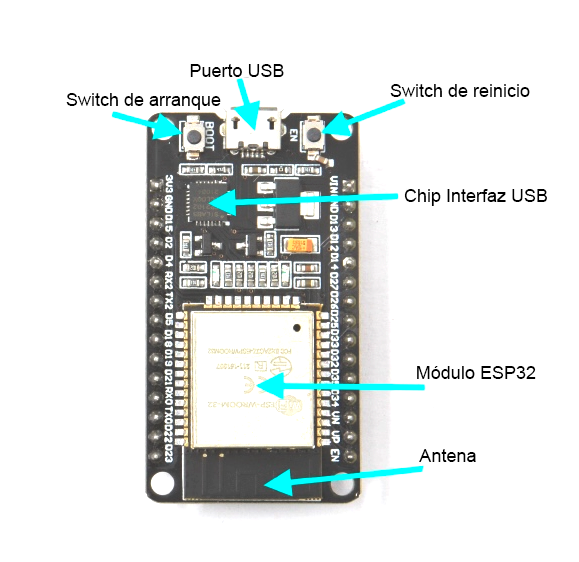
\includegraphics[width=0.45\linewidth]{tesis_fvalde/Imagenes/esp32.png}
    \caption{ESP32 Devkit 1}
    \label{fig:esp32}
\end{figure}

\begin{figure}[h!]
    \centering
    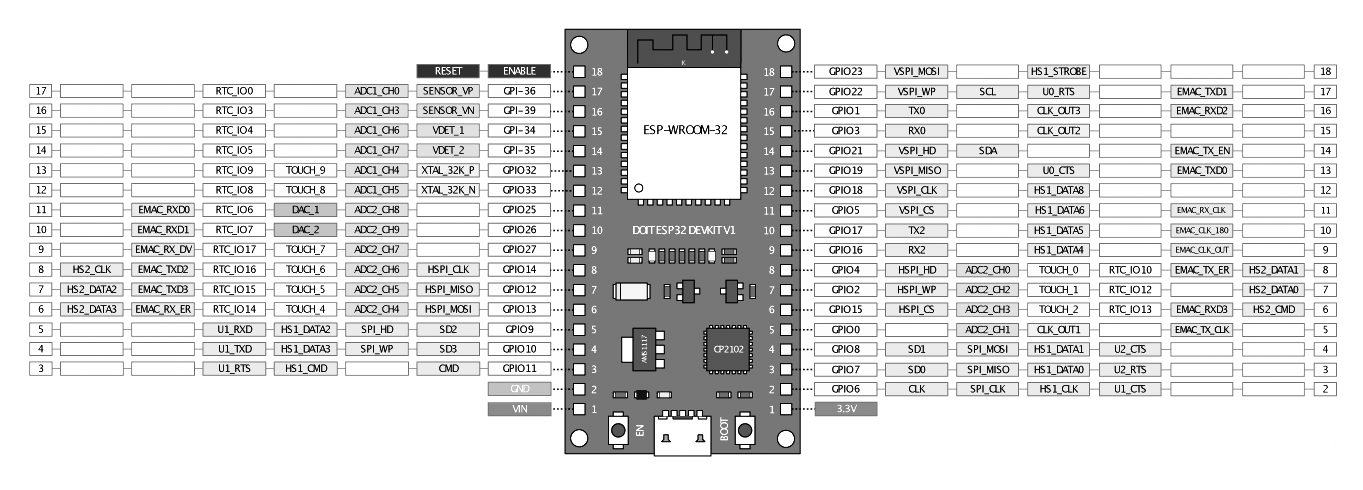
\includegraphics[width=0.98\linewidth]{tesis_fvalde/Imagenes/esp32pinoutx.png}
    \caption{Asignación de pines ESP32 DEVKIT V1}
    \label{fig:esp32pinout}
\end{figure}


\section{Módulo de radio RFM9x}

El módulo de radio RFM9x, desarrollado por la empresa HopeRF es un componente electrónico diseñado para la comunicación inalámbrica mediante la tecnología LoRa que provee una interfaz SPI (siglas en inglés de \textit{Serial Peripheral Interface}).

\vspace{0.5cm}

En la Figura 2.7 puede verse este módulo el cual se basa en el chip SX1276 que implementa la modulación LoRa y está optimizado para operar con un consumo de energía muy bajo. El RFM9x integra este chip simplificando su uso al eliminar la complejidad de su configuración.

\vspace{0.5cm}

\begin{figure}[h]
    \centering
    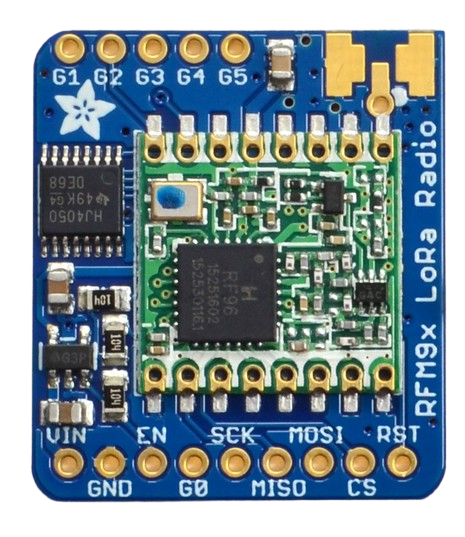
\includegraphics[height=0.25\linewidth]{tesis_fvalde/Imagenes/rfm9x.png}
    \caption{Módulo de radio RFM9x}
    \label{fig:adafruit-lora-RFM95W22}
\end{figure}

La comunicación entre el módulo de radio RFM9x y el ESP32 se basa en dos librerías, siendo la primera la \textit{RFM69 Library} para los módulos de radio RFM69W, RFM69HW, RFM69CW, RFM69HCW (para el chipset Semtech SX1231 y SX1231H) y la segunda es la librería \textit{RadioHead}, la cual es una librería de radio para microprocesadores de propósito general. 

\vspace{0.5cm}

Estos controladores (en inglés: \textit{device driver}, o simplemente \textit{driver}) son para su uso en el entorno de desarrollo de Arduino y MicroPython, las cuales no son compatibles con FreeRTOS ya que el driver no está listo para su uso en ESP-IDF, además el soporte para FreeRTOS en el entorno de desarrollo de Arduino está limitado para el ESP32 (\cite{ladyada2016}).

\vspace{0.5cm}

LoraLib (\cite{jangromes2020}) es otra librería para Arduino que ofrece soporte para diferentes chipsets LoRa, como el SX1278, SX1276, SX1277 y SX1279. Aunque este controlador ya no está en desarrollo activo, proporciona una capa de abstracción de hardware (HAL, siglas en inglés de \textit{Hardware Abstraction Layer}).

\vspace{0.5cm}

RadioLib utiliza el entorno de desarrollo de Arduino y se ejecuta en diferentes tipos de hardware, desde el ESP32, hasta el microcontrolador STM32 y/o Raspberry Pi (\cite{jangromes2024}). 

\vspace{0.5cm}

Si bien las librerías existentes ofrecen una buena base para la comunicación LoRa, presentan ciertas limitaciones que dificultan su integración en proyectos basados en ESP-IDF con soporte nativo para FreeRTOS, lo cual limita su uso en desarrollos con ESP32. 

\section{RTOS}

Un RTOS es un sistema operativo especializado diseñado para aplicaciones que requieren respuestas rápidas dentro de límites de tiempo estrictos. A diferencia de los sistemas operativos de propósito general, los RTOS priorizan la ejecución de tareas sobre otras, es decir, determina la importancia relativa de una tarea en relación a otras tareas y además cada una tiene una instantánea al momento de su ejecución con los valores que tenían los registros de memoria, información almacenada en la cola o variables globales, a esto se le conoce como contexto de ejecución.

\vspace{0.5cm}

Un RTOS proporciona mecanismos para que las tareas se comuniquen y se sincronicen, además de que están optimizados para un bajo consumo de recursos, lo que los hace ideales para sistemas embebidos (\cite{digikey_rtos}).

\subsection{FreeRTOS}

FreeRTOS es un RTOS hecho en colaboración con las principales empresas de chips del mundo quienes durante más de 15 años han colaborado en su desarrollo para microcontroladores y pequeños microprocesadores. Es distribuido gratuitamente bajo una licencia de código abierto, es decir, se pude descargar el código fuente y contribuir con cambios o mejoras. FreeRTOS incluye un núcleo y bibliotecas diseñadas para la confiabilidad y facilidad de uso.

\vspace{0.5cm}

Para poder utilizar FreeRTOS en el microcontrolador ESP32 es conveniente utilizar un conjunto de herramientas para comunicarse con la tarjeta de desarrollo. Debido a que el entorno de desarrollo ESP-IDF tiene su propia versión de FreeRTOS integrada como componente, se puede implementar programación de multiprocesador simétrico (SMP, siglas en inglés de \textit{Symmetric Multi-Processing}) que es cuando dos núcleos comparten acceso a la memoria principal, como es el caso del ESP32 (\cite{aws_freertos_esp32}).

\vspace{0.5cm}

FreeRTOS proporciona métodos para múltiples subprocesos, tareas y prioridad de las mismas. El énfasis está en la prioridad y velocidad de ejecución, por lo que no incorpora características que existen en otros sistemas operativos como el manejo de usuarios o redes. El núcleo del sistema son solo tres archivos en lenguaje C.

\vspace{0.5cm}

FreeRTOS se caracteriza por ser gratuito y distribuirse bajo la licencia MIT (siglas en inglés del \textit{Massachusetts Institute of Technology}), estar diseñado para dispositivos con microcontroladores para ser confiable y fácil de usar, implementarse en más de 40 arquitecturas y tener documentación colaborativa.